\section{Reasoning Framework Overview\label{sec:framework}}

The design goals of our framework are modularity for the
transformation steps and flexibility with respect to the underlying
inference engine. The modularity allows to reuse transformation
functionality across different WSML variants and reduces the effort
for accomplishing other reasoning tasks. By reducing WSML to simple
Datalog constructs and providing a respective object model we have
reduced the effort if integrating new reasoners to a minimum, in
fact the adaptation of the framework to the MINS rule engine took
less then a day.

\subsection{Architecture and Internal Layering}
Figure \ref{fig:layering} shows the basic components of the system
as well as the data flow during a prototypical usage scenario. The
inner box shows the currently implemented transformations that are
bundled to reduce the incoming WSML ontology to a Datalog program.
Different implementations of the ReasonerFacade provide the
translation of the simplified Datalog rules. Queries in fact use the
same infrastructure, except that a new set of transformation is
composed that neither includes the handling of constraints nor of
conceptual syntax.

{\bf HL: please correct the graphic, meta level axioms are injected
on the wsml level and not on the lower level!}

\begin{figure}[h]
    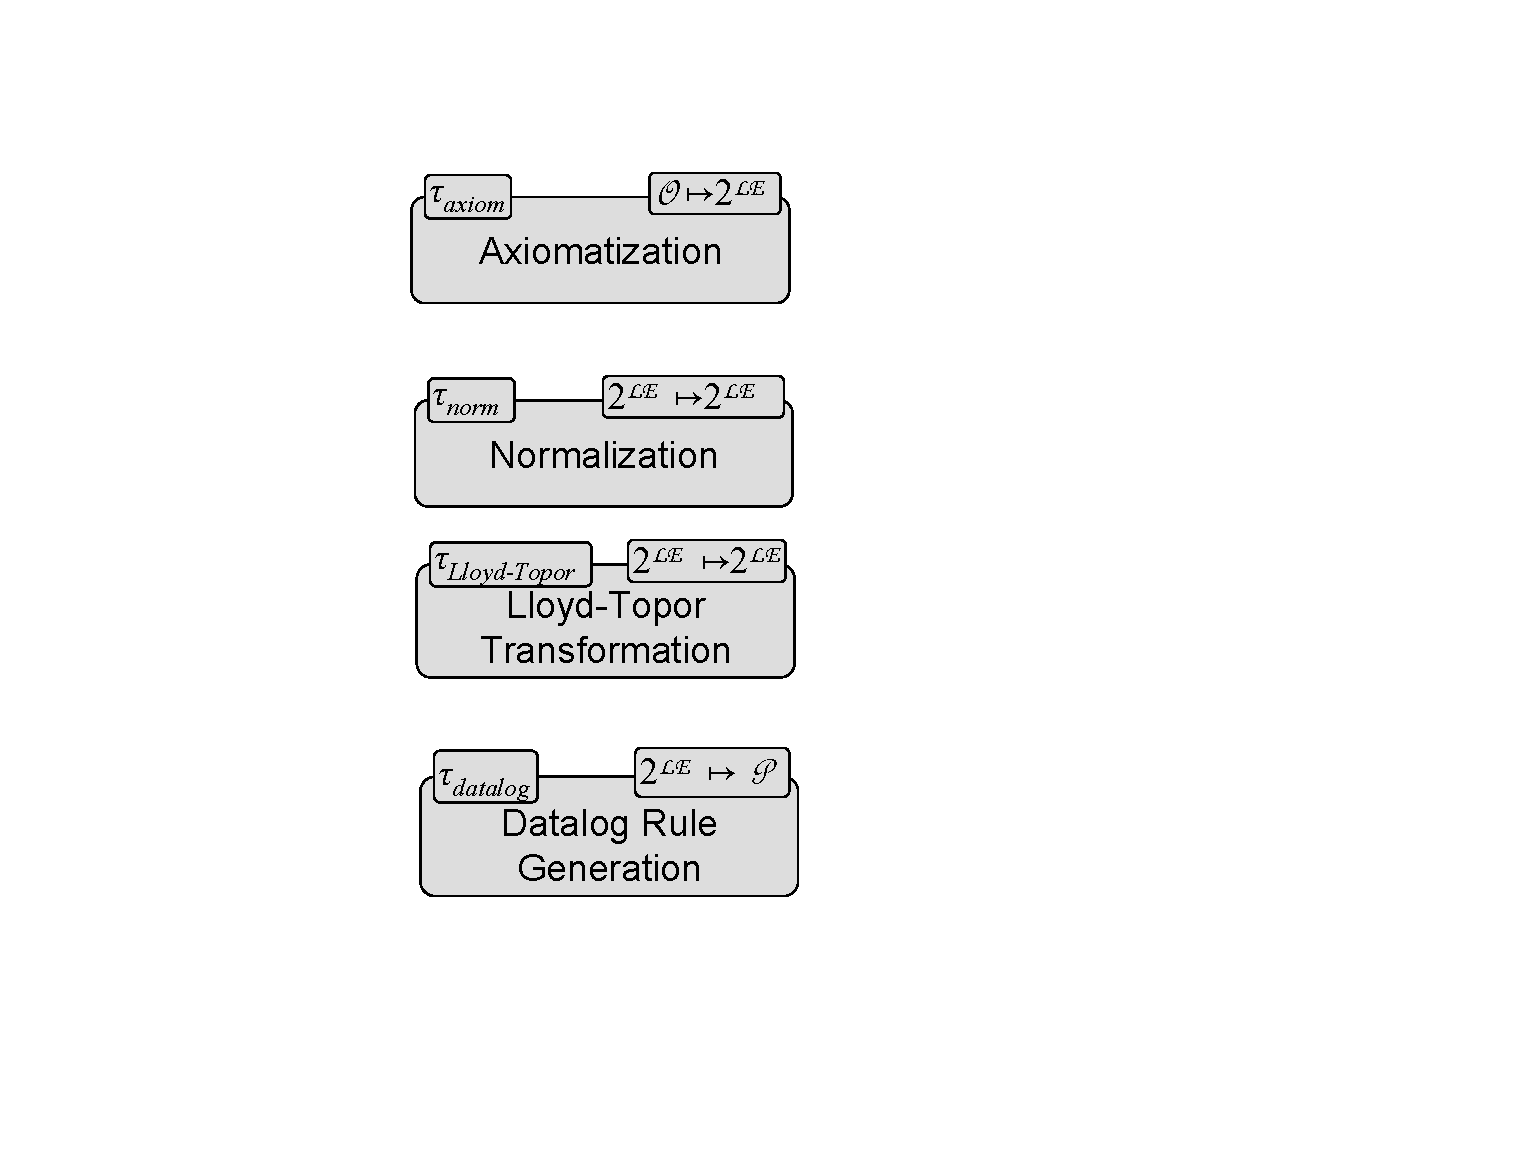
\includegraphics[width=11cm]{figures/layering}
    \centering
    \caption{Layering of the Internal Architecture. \label{fig:layering}}
\end{figure}


\subsection{Interface and Integration with Existing Technology}
So far we have not detailed on what data structure the framework
operates on. One could implement it directly with a parser and
compiler framework that generates some abstract syntax tree for WSML
which is directly transformed to the target format (Datalog).
Although this would have performance advantages it would greatly
reduce reusability and make maintenance harder. Our framework is
based on a intermediate object model of the language that is
provided by the WSMO4J\footnote{http://wsmo4j.sourceforge.net}
project. WSMO4J performs the task of parsing and validating the
input ontologies and provides the source object model for our
translations. In order to enable the usage of different Datalog
engines we additionally implemented a simple object model for
Datalog (Program, Rule) that is independent from any particular
engine.
